\documentclass[11pt]{article}

\usepackage{graphicx}
\usepackage[top=25mm, bottom=25mm, left=25mm, right=25mm, a4paper]{geometry}
\usepackage{amsmath}
\usepackage{enumitem}
\usepackage{float}
\usepackage{fancyhdr}
\usepackage{booktabs}
\usepackage{upquote}
\usepackage{tikz}
\usepackage{steinmetz}

\pagestyle{fancy}
\fancyhf{}
\fancyhead[R]{Baturay Kafkas - 2240357068 - Electrical \& Electronics Engineering}

\rfoot{\thepage}
\renewcommand{\headrulewidth}{0pt} 
\renewcommand{\footrulewidth}{0pt}
\sloppy

\begin{document}

\begin{center}
\large
\textbf{ELE228 - Programming for Circuits and Systems Preliminary Work 1}
\end{center}

\section{Questions}

\begin{enumerate}[leftmargin=*,label=\textbf{\arabic*.}]

\item Create a vector $\mathbf{t}$ between $0$ and $2\pi$ with $\pi/30$ intervals and form the following sinusoidal signals:
\[x(t)=16\sin^3(t)\]
\[y(t)=13\cos(t)-5\cos(2t)-2\cos(3t)-\cos(4t)\]

Plot the signals $x$ and $y$ on the same figure with respect to the vector $\mathbf{t}$. Make necessary adjustments so that you replicate \textit{Fig. 1} as closely as possible.

\item Consider the circuit in \textit{Fig. 2}. Obtain three independent equations for the voltages $V_1, V_2$, and $V_3$ using the node-voltage approach. Solve for the node-voltages on paper using your preferred method, such as Gaussian elimination or matrix inversion.

\item  Consider the circuit in \textit{Fig. 2} again. Arrange the node-voltage equations you wrote in the previous part in matrix form as
\[A\mathbf{V}=\mathbf{b}\]

where $A$ is the coefficient matrix, $\mathbf{V}$ is the vector containing the unknown node voltages $V_1, V_2$, and $V_3$ and $\mathbf{b}$ is the vector of independent current sources. Solve for $\mathbf{V}$ using MATLAB and compare the result with your result from the previous part.

\begin{figure}[H]
    \centering
    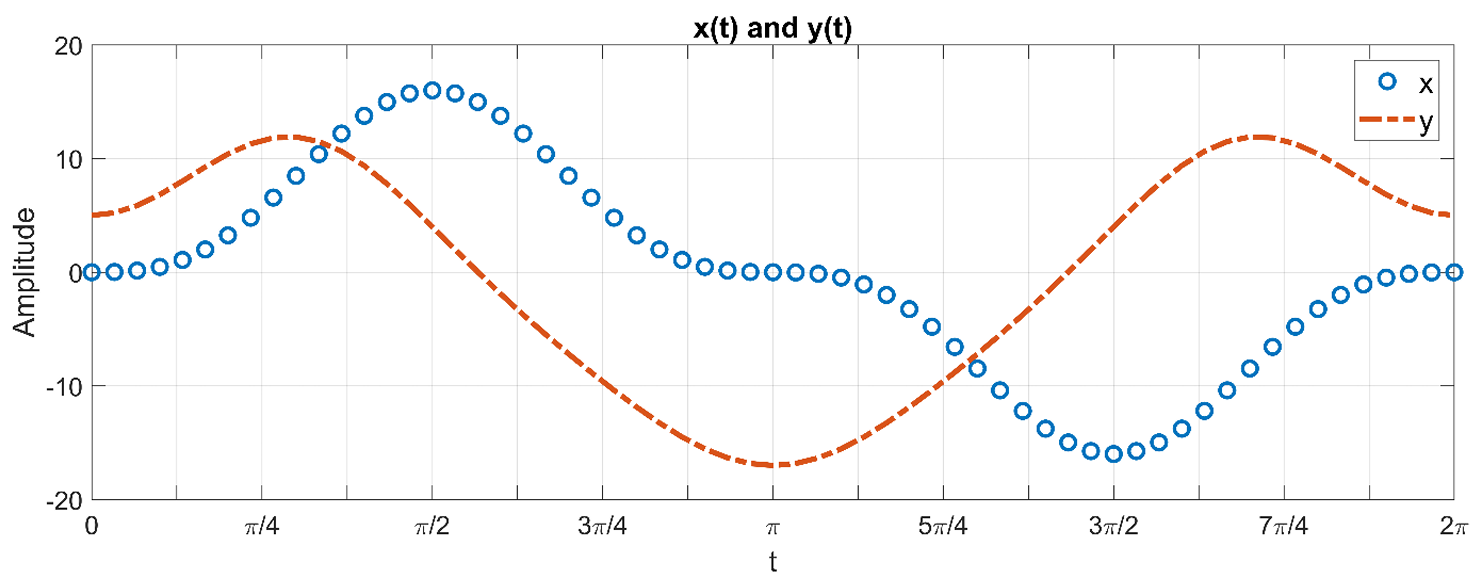
\includegraphics[width=1\linewidth]{msedge_2schueYzXs.png}
    
    \textit{Figure 1}
    
    \vspace{2em}
    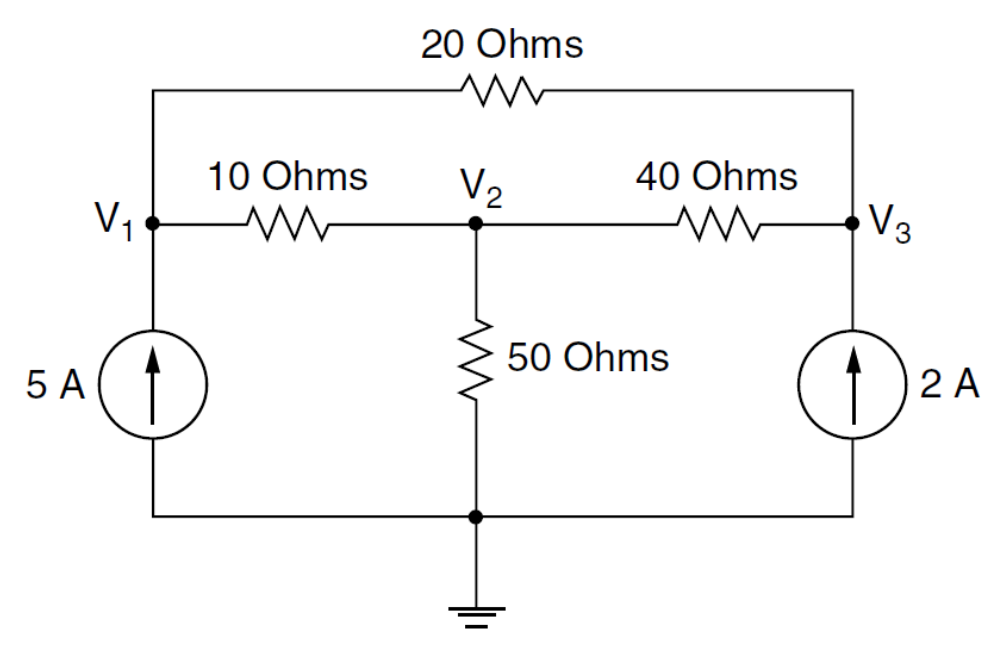
\includegraphics[width=0.5\linewidth]{chrome_wD5aFGZ7Oh.png}
        
    \textit{Figure 2}
\end{figure}

\end{enumerate}

\newpage

\section{Answers}

\begin{enumerate}[leftmargin=*,label=\textbf{\arabic*.}]

\item Code:

\vspace{1em}

\hrule
\begin{verbatim}
t = 0:pi/30:2*pi
x = 16*sin(t).^3
y = 13*cos(t)-5*cos(2*t)-2*cos(3*t)-cos(4*t)

set(gca,'TickLabelInterpreter','latex')
grid on
hold on
box on

plot(t, x, 'bo')
plot(t, y, 'r-.','LineWidth', 1.5)
xticks(0:pi/8:2*pi)
xticklabels({'$0$','','$\pi/4$','','$\pi/2$','','$3\pi/4$','', ...
    '$\pi$','','$5\pi/4$','','$3\pi/2$','','$7\pi/4$','','$2\pi$'})
yticks(-20:10:20)
xlim([0 2*pi])
ylim([-20 20])
legend('x','y')
xlabel('t', Interpreter='latex')
ylabel('Amplitude', Interpreter='latex')
title('\bf{x(t) and y(t)}', Interpreter='latex')

hold off
saveas(gca, 'fig1.png')
\end{verbatim}
\hrule

\vspace{1em}

Figure:

\begin{figure}[H]
    \centering
    
\includegraphics[width=1\linewidth]{fig1.png}
\end{figure}

\item Obtain the node-voltage equations.

Node $V_1$:
\begin{align}
\frac{V_1 - V_2}{10} + \frac{V_1 - V_3}{20} &= 5 \nonumber\\
3V_1 - 2V_2 - V_3 &= 100
\end{align}
Node $V_2$:
\begin{align}
\frac{V_2 - V_1}{10} + \frac{V_2 - V_3}{40} + \frac{V_2}{50} &= 0 \nonumber\\
-20V_1 + 29V_2 - 5V_3 &= 0
\end{align}

Node $V_3$:
\begin{align}
\frac{V_3 - V_1}{20} + \frac{V_3 - V_2}{40} &= 2 \nonumber\\
-2V_1 - V_2 + 3V_3 &= 80
\end{align}

The matrix form using $(1), (2),$ and $(3)$:
\[
\underbrace{\begin{bmatrix}
3 & -2 & -1 \\
-20 & 29 & -5 \\
-2 & -1 & 3
\end{bmatrix}}_A
\underbrace{\begin{bmatrix}
V_1 \\
V_2 \\
V_3
\end{bmatrix}}_\mathbf{V}
=
\underbrace{\begin{bmatrix}
100 \\
0 \\
80
\end{bmatrix}}_\mathbf{b},
\]

where $\mathbf{V}=[V_1\quad V_2\quad V_3]^T$. Check if the determinant is non-zero so that the matrix is invertible.
\[|A| =
\begin{vmatrix}
3 & -2 & -1 \\
-20 & 29 & -5 \\
-2 & -1 & 3
\end{vmatrix}
=
3
\begin{vmatrix}
29 & -5 \\
-1 & 3
\end{vmatrix}
+ 2
\begin{vmatrix}
-20 & -5 \\
-2 & 3
\end{vmatrix}
- 1
\begin{vmatrix}
-20 & 29 \\
-2 & -1
\end{vmatrix}=28\neq0
\]
\[A\mathbf{V}=\mathbf{b}\implies\mathbf{V}=A^{-1}\mathbf{b}\]

Calculate the inverse of $A$ using the cofactor method.

\[A^{-1}=\frac1{\det A}\underbrace{\begin{bmatrix}
\begin{vmatrix}29 & -5 \\ -1  & 3\end{vmatrix} & -\begin{vmatrix}-2 & -1 \\ -1  & 3\end{vmatrix} & \begin{vmatrix}-2 & -1 \\ 29  & -5\end{vmatrix} \\[1em]
-\begin{vmatrix}-20 & -5 \\ -2  & 3\end{vmatrix} & \begin{vmatrix}3 & -1 \\ -2  & 3\end{vmatrix} & -\begin{vmatrix}3 & -1 \\ -20  & -5\end{vmatrix} \\[1em]
\begin{vmatrix}-20 & 29 \\ -2  & -1\end{vmatrix} & -\begin{vmatrix}3 & -2 \\ -2  & -1\end{vmatrix} & \begin{vmatrix}3 & -2 \\ -20  & 29\end{vmatrix}
\end{bmatrix}}_{\text{adj}\,A}=\frac{1}{28}
\begin{bmatrix}
82 & 7 & 39 \\
70 & 7 & 35 \\
78 & 7 & 47
\end{bmatrix}
\]
\[\mathbf{V}=A^{-1}\mathbf{b}=\frac{1}{28}
\begin{bmatrix}
82 & 7 & 39 \\
70 & 7 & 35 \\
78 & 7 & 47
\end{bmatrix}\begin{bmatrix}
100 \\
0 \\
80
\end{bmatrix}=\begin{bmatrix}
404.29\text{ V}\\ 350 \text{ V}\\412.86\text{ V}
\end{bmatrix}\]

Therefore, $V_1=404.29 \text{ V},\: V_2=350\text{ V},\: V_3=412.86 \text{ V}$.

\item Code:

\vspace{1em}

\hrule
\begin{verbatim}
A = [3 -2 -1; -20 29 -5; -2 -1 3]
b = [100; 0; 80]
V = A\b
\end{verbatim}
\hrule

\begin{figure}[H]
\hspace{1em}
    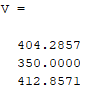
\includegraphics[width=0.14\linewidth]{dxSPKmdpF5.png}
\end{figure}

\end{enumerate}

The result obtained in Question 2 is consistent with the one in Question 3.
\end{document}